\documentclass[a4paper,10pt]{article}
\usepackage[utf8]{inputenc}

\usepackage{graphicx} % Allows including images
\usepackage{booktabs} % Allows the use of \toprule, \midrule and \bottomrule in tables
%\usepackage{hyperref} % Allows to put hyperlinks.
\usepackage{color}
\usepackage{listings}
\usepackage[english]{babel}
\usepackage{subcaption}
\usepackage{float}
\usepackage{amsmath}
\usepackage[hidelinks]{hyperref}
%opening
\title{Hilbert curve based flexible dynamic partitioning scheme for adaptive scientific computations}
\author{Hari Sundar, Milinda Fernando}
\date{}

\begin{document}

\maketitle

\begin{abstract}
In this paper we present a Hilbert curve based flexible dynamic partitioning scheme for adaptive scientific computations. Unlike most partitioning schemes our approach is not focused on perfect load
balancing, which can increase communication costs. Instead of traditional approach, we introduce some flexibility (slack) to the load at each node, reducing the communication costs further. Our results
show that load balancing with some flexibility allowed is [xx]\% efficient than the traditional partitioning approaches and it can reduce the overall computation time by [xx]\%.We use Hilbert curve instead
of commonly used Morton curve in order to preserve the geometric locality more efficiently. Since, current implementations of Hilbert curve computations are expensive, we propose a new algorithm that works
for all SFC using the property of the NCA. Our results show that the NCA based Hilbert ordering computation is [XX] times faster than the traditional recursive approach. 
\end{abstract}

\section{Introduction}
Load balancing and partitioning are critical when it comes to parallel computations. Generally partitioning involves the tasks of equally dividing the work and data among the processors,
reducing processor idle time and the communication costs. Partitioning can be done statically or dynamically. In this research we are focused on developing an efficient flexible dynamic
partitioning scheme based on Space Filling Curves (SFC) which mostly suites for adaptive computations. Unlike most partitioning schemes , we are not focused on achieving the
perfect equal load balancing which can increase the communication costs. Our approach allows some flexibility to the load, that each node gets (near perfect equal load balancing) which
empirically shown to reduce the communication costs and overall computation time. One of the main advantage of SFC based partitioning (compared to graph based partitioning) is,
preservation of geometric locality of objects between processors. Depending on the SFC (i.e. Morton, Peano,Hilbert) that used for partitioning, the amount of locality preserved differs. 
Most of the SFC based partitioning use the Morton curve which is good for current range of clusters in terms of giving good load balance, but as we focus on larger levels of parallelism,
we show that Hilbert will be more effective. Recursive computation of Hilbert ordering can be inefficient partitioning large tasks, which can lead to low performance in overall computation.
In this paper we present an approach based on Nearest common Ancestor (NCA) which can be extended to calculate any SFC ordering efficiently. Considering the results we gathered we can show that
the Hilbert ordering based on NCA, is [xx] times faster than the traditional recursive approach.

\section{Related Work}

\section{Methodology}

\subsection{Allowing flexibility in dynamic load balancing}

As mentioned earlier most of the partitioning schemes are focused on uniform distribution of tasks across all the processor. The main drawback of this approach is, the uniform load balancing can cause
increased communication costs, slowing down the overall computation. In this paper we introduce some flexibility to the load balancing (i.e near uniform load balancing) in order to reduce the communication
costs and improve the overall execution time of the computation. To demonstrate the above claim we conduct two experiments.
\begin{itemize}
 \item Standard SFC based partition, where the work is uniform across all processes and compare the communication (using the surface area of the partition as a surrogate)
 \item A flexible SFC based partition, where we allow a small 'slack' (flexibility) in the amount of work that each process gets in order to reduce the communication costs. 
\end{itemize}

Since most of the current implementations (i.e. recursive approach) of Hilbert curve are expensive in computation and does not suite for dynamic load balancing. To over come that we present an efficient
way to calculate Hilbert ordering based on the Nearest Common Ancestor (NCA), described in the following section. 


\subsection{Space Filling Curve (SFC) ordering based on Nearest Common Ancestor (NCA)}
SFC is a surjective mapping between the one dimensional space to higher dimensional space. Generally almost all the SFC adhere to the recursive nature in curve generation. Because of the recursive
nature SFCs have, most of the SFCs can be computed recursively. In this paper we present an algorithm to compute Hilbert ordering based on the NCA which is xx\% efficient than the recursive approach.
The main advantage of the NCA based Hilbert ordering calculation is the extensibility of the algorithm for other SFCs. Using the NCA property, any SFC ordering can be easily computed. The key idea of
the NCA based approach is, regardless of the SFC that we consider, we find the NCA for a given two coordinates (see figure \ref{NCA}).  As the next step we need to figure out the rotation pattern inside the NCA element. Since
the rotation pattern in fine cell depends on the rotation patterns of more grain cells (i.e in Hilbert curve) we traverse the octree from root to NCA once figuring out the rotation pattern inside the NCA. 

\begin{figure}[H]
\centering
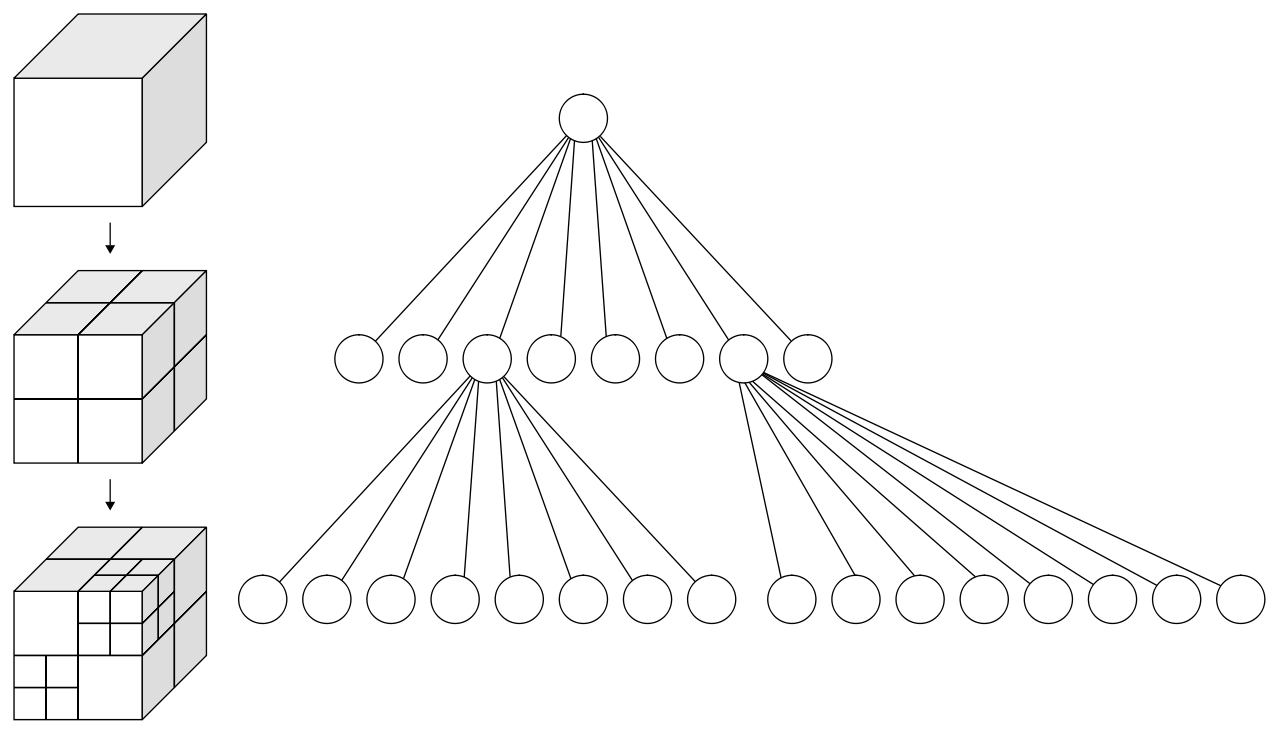
\includegraphics[height=40mm,keepaspectratio]{images/NCA.png}
\caption{Nearest Common Ancestor (NCA) of a octree \label{NCA}}
\end{figure}


\par

Even though there are multiple SFCs available, we mainly focus on the Morton and Hilbert curves and their ordering computations. To compare the NCA based ordering approach with other approaches we have
implemented both Hilbert and Morton as following.
\begin{itemize}
 \item Hilbert ordering baseline implementation (Implementation based on recursive approach)
 \item Morton ordering baseline implementation (Implementation based on non-recursive approach (i.e current implementation in dendro[reference]))
 \item Hilbert ordering NCA implementation (Implementation based on NCA calculation)
 \item Morton ordering NCA implementation (Implementation based on NCA calculation)
\end{itemize}

\section{Results}

Baseline and NCA based Hilbert and Morton ordering algorithms are executed with varying maximum depth for sorting one million (2D \& 3D) points. In this context maximum depth refer to the maximum height of the
octree needed to compute the Hilbert or Morton ordering. Each implementation of the Hilbert and Morton ordering executed twenty times and mean executing time in milliseconds is taken as the performance measure.
Fig.\ref{2d} and Fig.\ref{3d} depict the 2D and 3D Hilbert and Morton ordering performance for different implementations. All the SFC implementations are run in the following experimental setup.

\begin{itemize}
 \item Intel Xeon E7-4820v2 CPU @2.00 GHz (32 cores)
 \item RAM: 64 GB DDR3
 \item OS: Ubuntu 14.04 LTS
 \item Compiler: g++ 4.8
\end{itemize}


\begin{figure}[H]
\centering
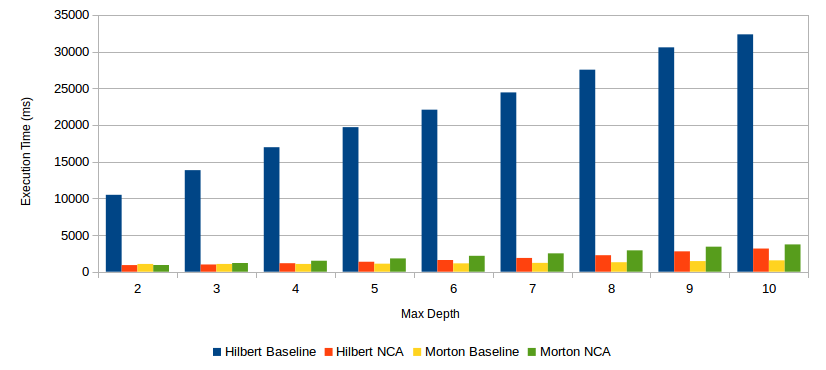
\includegraphics[height=50mm,keepaspectratio]{images/2d.png}
\caption{Hilbert and Morton ordering (2D coordinates) performance \label{2d}}
\end{figure}

\begin{figure}[H]
\centering
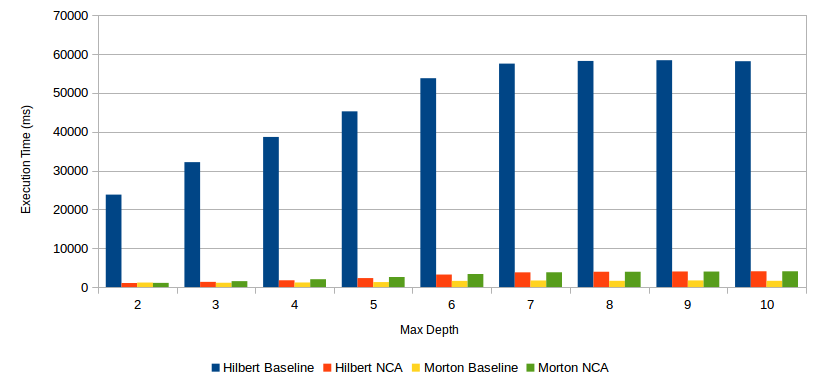
\includegraphics[height=50mm,keepaspectratio]{images/3d.png}
\caption{Hilbert and Morton ordering (3D coordinates) performance for different implementations \label{3d}}
\end{figure}


\section{Conclusion}


\end{document}
